\documentclass{standalone}
\begin{document}

Une importante part des problèmes modernes se ramène à l'étude de graphes. En particulier, la grande majorité des données et traces liées aux activités humaines peuvent être modélisés par des réseaux, des relations ou des circuits. Que ce soit les réseaux informatiques -- centralisés ou pair à pairs -- ou plus simplement les interactions ou liens sociaux, toutes ces données peuvent l'objet de recherche de communautés. La recherche de communautés a des applications pour les études sociologiques et les analyses socio-économiques. Un exemple original est celui de l'identification d'utilisateurs du \emph{Bitcoin}. Si c'est a priori un système anonyme, il n'en reste pas moins que par principe, la \emph{blockchain} rend publics toutes les transactions et tous les échanges. Il est possible pour n'importe qui de les étudier. L'anonymat provient du fait que chacun peut se créer autant de \textit{comptes} qu'il le souhaite, et ensuite effectuer des transactions entre ses propres comptes pour rappatrier l'argent là où il le souhaite. Néanmoins, en étudiant le graphe, dont les sommets sont les comptes et les arêtes les transactions, de reconstruire les communautés d'échanges et identifier des acteurs, des groupes de comptes appartenant à une unique entité etc...~\cite{bitcoin}.

Dans ce cours, nous allons plus particulièrement étudier le problème de reconstruction exacte de communauté~\cite{dyier}, c'est à dire, en supposant l'existence de deux communautés sous-jacentes, de tailles égales conditionnant la construction du graphe de relations entre les individus, retrouver ces deux communautés en étudiant uniquement le graphe induit. Nous nous ramèneront à un problème de partitionnement de graphe courant mais $\NPHARD$: le problème de la bissection minimale. 

Pour étudier le problème de reconstruction exacte de communautés dans un graphe nous définirons tout d'abord un modèle de graphe aléatoire modélisant les graphes induits par deux communautés pré-établies. Puis nous donnerons une méthode reconstruction exacte avec grande probabilité de ces communautés avant d'en étudier en détail la classe de complexité algorithmique. Plus précisément, nous montrerons qu'une bissection minimale du graphe est solution du problème de reconstruction exacte avec grande probabilité mais que la recherche d'une telle bissection est un problème $\NPCOMPLETE$.
	
\subsection{Modèle}
	\subsubsection{Construction de graphe}
	
	\begin{defn}[Modèle 1]
		\label{model}
		L'objectif est de construire un graphe aléatoire $G=(V,E)$. On se donne $V = \set{1, \cdots, 2N}$ un ensemble, $p, p_A, p_B \in [0,1]$ des probabilités. On suppose qu'on dispose de $A \subset V$, tel que $\card{A} = N$ construit  aléatoirement et on note $B = V \backslash A$. On alors: $V = A \sqcup B$ $\card{B} = \card{A} = N$.
		
		On définit $\sigma:\; V \longrightarrow \set{-1, 1}$ la fonction d'étiquetage des sommets telle que:		
		\[ 
		\forall v \in V,\, \sigma(v) = \left\{ \begin{array}{lr}
			1& \text{si } v \in A\\
			-1& \text{si } v \in B
		\end{array}\right.
		\]		
		On alors les arêtes de $E$ de la façon suivante pour tout $(u,v) \in V^2$.
		\[
		\Proba[(u,v) \in E] = \left\{ \begin{array}{lr}
		p& \text{si } \sigma(u) \not= \sigma(v)\\
		p_A& \text{si } u,v \in A\\
		p_B& \text{si } u,v \in B
		\end{array}\right.
		\]		
		Dans la suite on notera $G \follows \Ger(N, p_A, p_B, p)$, $G$ est un graphe aléatoire construit selon ce modèle.
	\end{defn}
	
	\subsubsection{Exemples}
	
	\begin{figure}[H]
		\centering
		\begin{subfigure}{0.3\textwidth}
			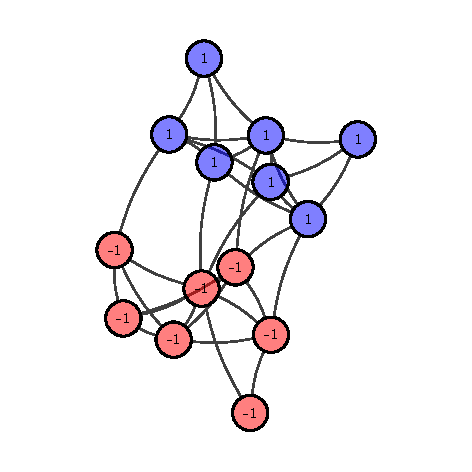
\includegraphics[scale=0.5]{ig-plots/tmp/large_inter_proba.pdf}
			\caption{$p_A = p_B = 0.8, p=0.1$}
		\end{subfigure}
		\begin{subfigure}{0.3\textwidth}
			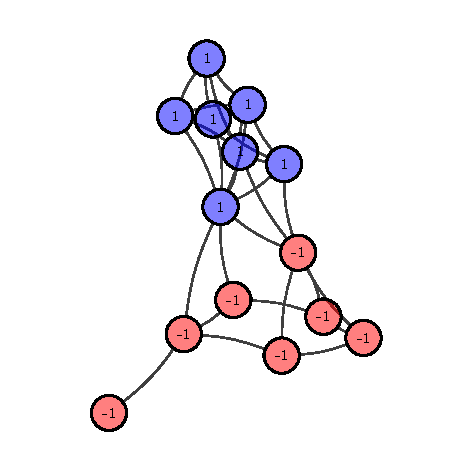
\includegraphics[scale=0.5]{ig-plots/tmp/large_small_smaller.pdf}
			\caption{$p_A = 0.9, p_B = 0.3, p=0.05$}
		\end{subfigure}
		\begin{subfigure}{0.3\textwidth}
			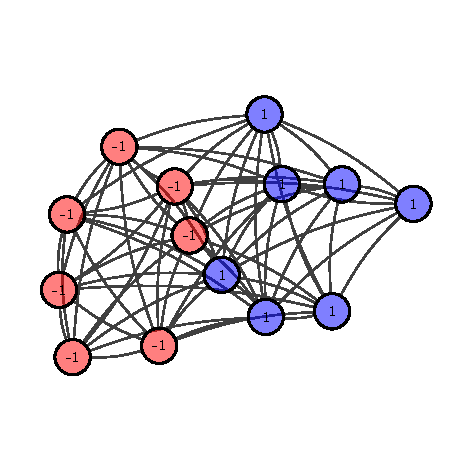
\includegraphics[scale=0.5]{ig-plots/tmp/large_largenoise.pdf}
			\caption{$p_A = p_B = 0.9, p=0.5$}
		\end{subfigure}
		
		
		
		\caption{Exemples de graphes générés par le modèle avec différents paramètres}
	\end{figure}

\subsection{Problème de reconstruction exacte}
	Soient $A,B$ deux ensembles de tailles égales, on suppose avoir un graphe $G \follows \Ger(N, p_A, p_B, p)$ le graphe induit par les deux communautés $A$ et $B$. On note $\sigma$ la fonction d'étiquetage associée. On définit formellement le problème que l'on cherche à résoudre.
	
	\begin{defn}[Problème de reconstruction exacte]
		On cherche à reconstruire $\sigma$ en l'estimant à partir de l'observation du graphe. Le problème revient à construire $\hat{\sigma}$ tel que:
		\[ \Proba[\hat{\sigma} = \pm \sigma] \underset{N \rightarrow \infty}{\longrightarrow} 1
		\]
		On cherche $\sigma$ au signe prêt car on cherche seulement à retrouver les deux communautés, peu importe leur étiquetage original: on cherche $A$ et $B$ à renommage près.
	\end{defn}

	Nous allons examiner une solution particulière: la bissection minimale du graphe. Nous montrerons qu'elle correspond à la solution cherchée avec grande probabilité.

\subsection{Bissection minimale}

	\begin{defn}[Bissection et coupe]
		Soit $G=(V, E)$ un graphe. Une coupe de $G$ est une partition des sommets en deux ensembles $(A, B)$. Une bissection de $G$ est une coupe $(A,B)$ de $G$ avec $\card{A} = \card{B}$.
		
		On notera $(A:B)$ pour parler de la coupe (ou de la bissection, suivant le contexte) $(A,B)$. Par abus de notations on considérera que $(A:B)$ désigne aussi l'ensemble des arêtes dont une extrémité est dans $A$ et l'autre dans $B$.
	\end{defn}

	\begin{rem}
		Par la suite on utilisera la notation $(A:B)$ pour introduire la coupe d'ensembles $A, B$: $V = A \sqcup B$.
		On parlera par la suite de la bissection ou de la coupe $(A:B)$ suivant si $A$ et $B$ sont de tailles égales ou non.
	\end{rem}

	\begin{defn}[Flot]
		Soient $G = (V, E)$ et $A, B \subset V$ disjoints. On appelle flot entre $A$ et $B$ la somme des capacités des arêtes dont une extrémité est dans $A$ et l'autre dans $B$. 
		
		On note cette valeur $\card{A:B}$. En effet, dans le cas d'un graphe non pondéré, le flot correspond au cardinal de $(A:B)$.
	\end{defn}

	\begin{defn}[Ordre sur les bissections]
		Soit $G=(V, E)$, et $(A:B)$, $(A':B')$ deux bissections de G.
		On dit que $(A:B) \preceq A':'B$ si et seulement $\card{A:B} \leq \card{A':B'}$.
		
		Autrement dit, une bissection est plus petite qu'une autre si le flot
	\end{defn}

	Dans la suite on va étudier l'existence et la recherche des bissections minimales pour $\preceq$ d'un graphe. Il se trouve que le cadre du modèle \ref{model} précédemment énoncé, la bissection minimale est presque sûrement solution du problème de reconstruction exacte~\cite{dyier}. Dans la section suivante nous allons voir la preuve de ce résultat avant d'analyser la complexité du problème de a bissection minimale d'un graphe~\cite{simplenphard}.

\end{document}
